%The goal of this section is to (i) explain the experimental setup, (ii) demonstrate the effectiveness of \scheme\ in synthesizing
%different programs, and (iii) analyze its running time.

%\subsection{Experimental Setup}
%\label{sec-setup}

\subsection{\scheme\ Results}
\label{sec-effectiveness}
As shown in Figure~\ref{fig_loss}, both train and validation losses are improved at some point after 7th sub-data iteration. However, as training reaches the end of our dataset, at around 20th sub-data iterations, we observe spikes of loss increases which may be due to overfitting of the data. To achieve a high accuracy with time series with greater sizes, we will need further hyperparameter tuning to complement this by, for example, adjusting threshold to create signals in our wavelet transformer. 



\begin{figure}[htpb]
\begin{center}
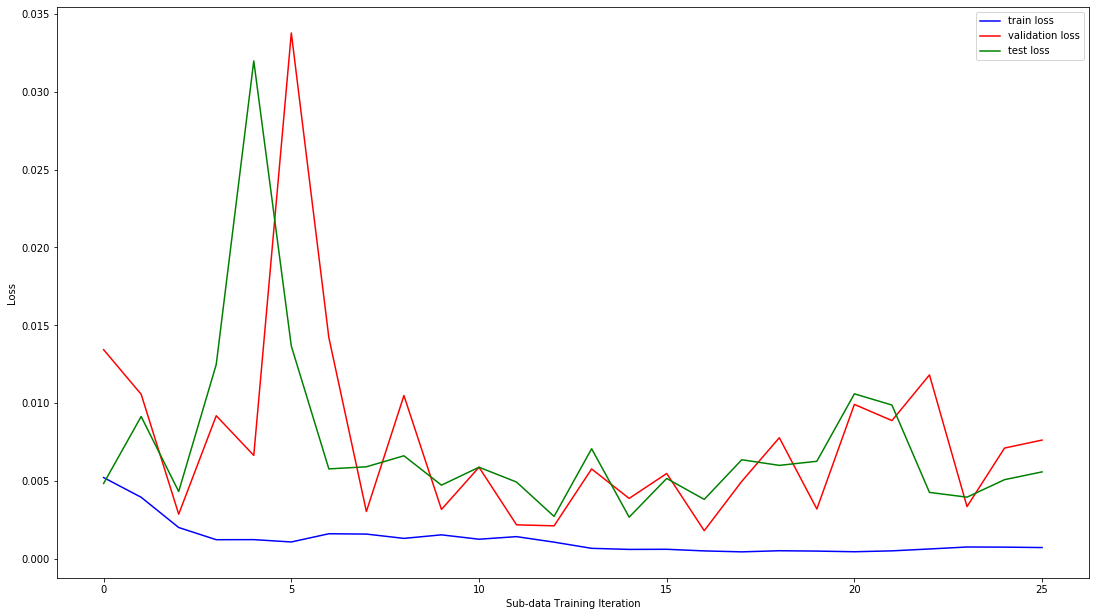
\includegraphics[width=0.9\textwidth]{./figs/lossvsiter}
\vspace{-0.2cm}
\caption{Loss per Sub-dataset Training Iteration}
\label{fig_loss}
\end{center}
\vspace{-0.4cm}
\end{figure}

The actual and predicted price data for S\&P500 are shown in Fig~\ref{fig_loss} and Fig~\ref{fig_actual}. Our model predicts S\&P500 index with reasonable accuracies as shown in Figure~\ref{fig_diff}. At the start, the differences of predicted and actual prices are negligible. However, we observe exponential increase of inaccuracy of over 10 percent of the prices when the stock price plummeted at 2,500 to 3,000th timeframes. The model’s accuracy dropping when the market sentiment is low is further proven by the most recent drop of index prices at around 4,700th timeframe. 

Regarding our model and training schemes, we discovered normalization worsens accuracy compared to when features are scaled manually. We think that this is accountable by that train and test set are normalized at the same time. In other words, there are potential leaks of future information in each time step. Regarding the stacked autoencoder, the intuition was to derive hidden deep features out of the original raw dataset. However, what we think it actually does is to force our data into smaller dimensions with potential loss of important information. We will conduct accuracy comparison with the model without SAE in the future. 

\begin{figure}[htpb]
\begin{center}
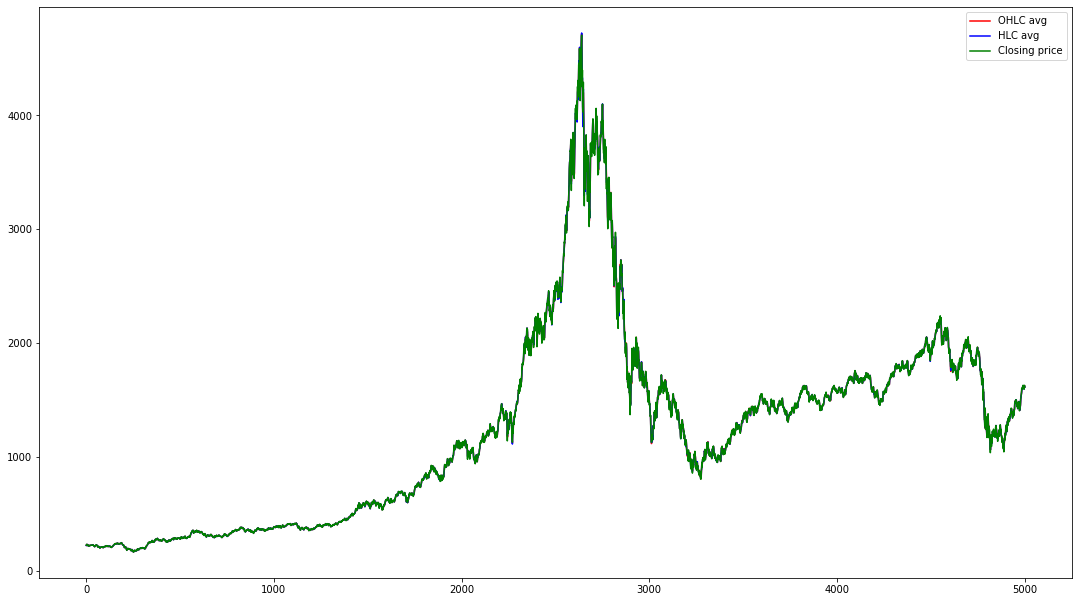
\includegraphics[width=0.9\textwidth]{./figs/actualprice}
\vspace{-0.2cm}
\caption{Actual Data}
%\todo{fix scale from 1 to 41 and 1 to 100}}
\label{fig_actual}
\end{center}
\vspace{-0.6cm}
\end{figure}

\begin{figure}[htpb]
\begin{center}
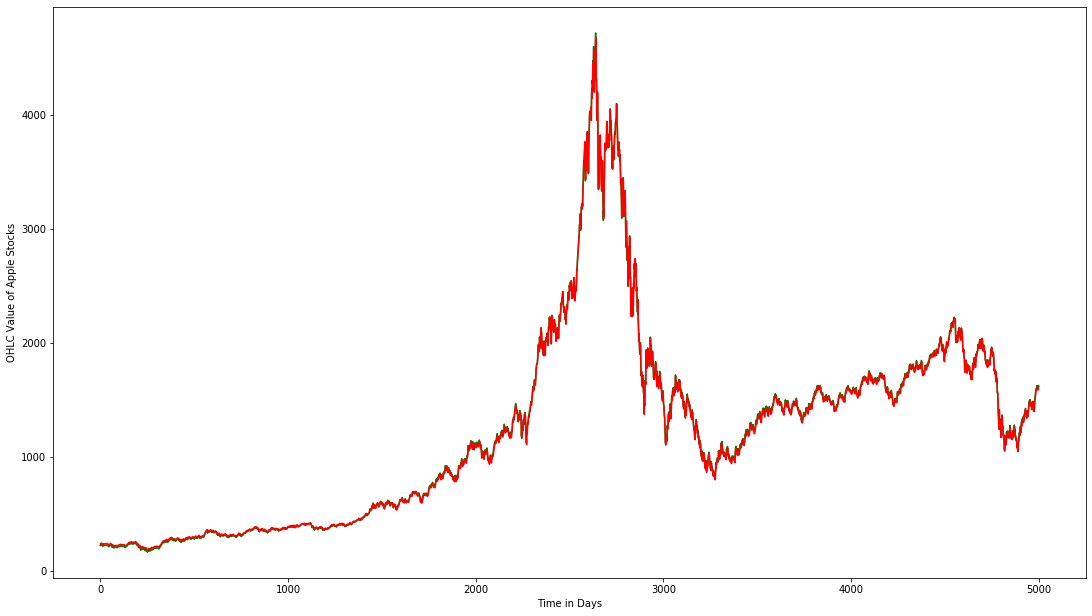
\includegraphics[width=0.9\textwidth]{./figs/predictedprice}
\vspace{-0.2cm}
\caption{Predicted Data}
%\todo{fix scale from 1 to 41 and 1 to 100}}
\label{fig_predict}
\end{center}
\vspace{-0.6cm}
\end{figure}



\begin{figure}[htpb]
\begin{center}
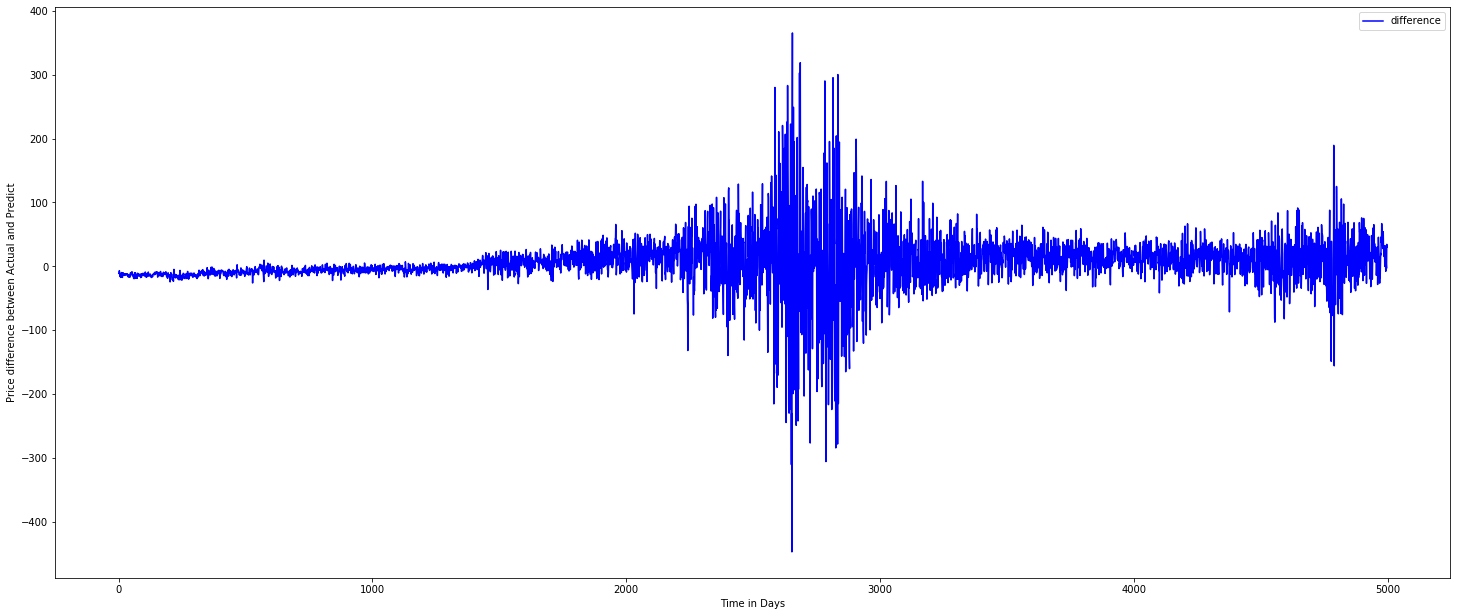
\includegraphics[width=0.9\textwidth]{./figs/pricediff}
\vspace{-0.2cm}
\caption{Difference between Predicted and Actual Prices}
%\todo{fix scale from 1 to 41 and 1 to 100}}
\label{fig_diff}
\end{center}
\vspace{-0.6cm}
\end{figure}



Besides, we tested price history using point-by-point approach and sequence-by-sequence approach in our second architecture. The training and test rate is 0.8. We found that by using 8 epoch, we can achieve the accuracy at 60\%. Though we can find some trends by using the sequence by sequence, the prediction is not stable (Figure 11&12). The point by point prediction figures looks very good but here it is a bit deceptive. We can only predict one data point ahead, based on its all previous history.

\begin{figure}[htpb]
\begin{center}
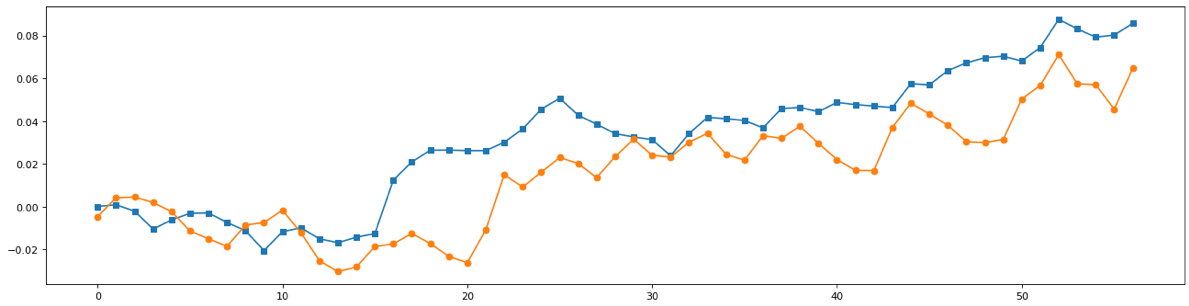
\includegraphics[width=0.9\textwidth]{./figs/PP_2_50.PNG}
\vspace{-0.2cm}
\caption{Point-by-Point prediction (2 Epoch, 50 Batch size)}
%\todo{fix scale from 1 to 41 and 1 to 100}}
\label{fig_predict}
\end{center}
\vspace{-0.6cm}
\end{figure}

\begin{figure}[htpb]
\begin{center}
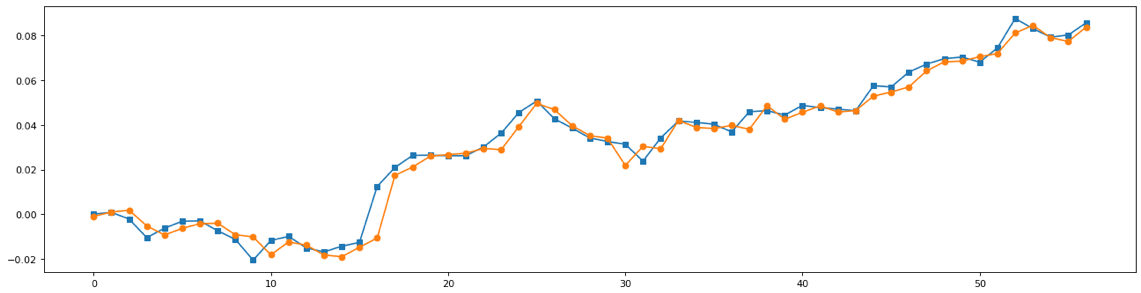
\includegraphics[width=0.9\textwidth]{./figs/PP_8_50.PNG}
\vspace{-0.2cm}
\caption{Point-by-Point prediction (8 Epoch, 50 Batch size)}
%\todo{fix scale from 1 to 41 and 1 to 100}}
\label{fig_predict}
\end{center}
\vspace{-0.6cm}
\end{figure}

\begin{figure}[htpb]
\begin{center}
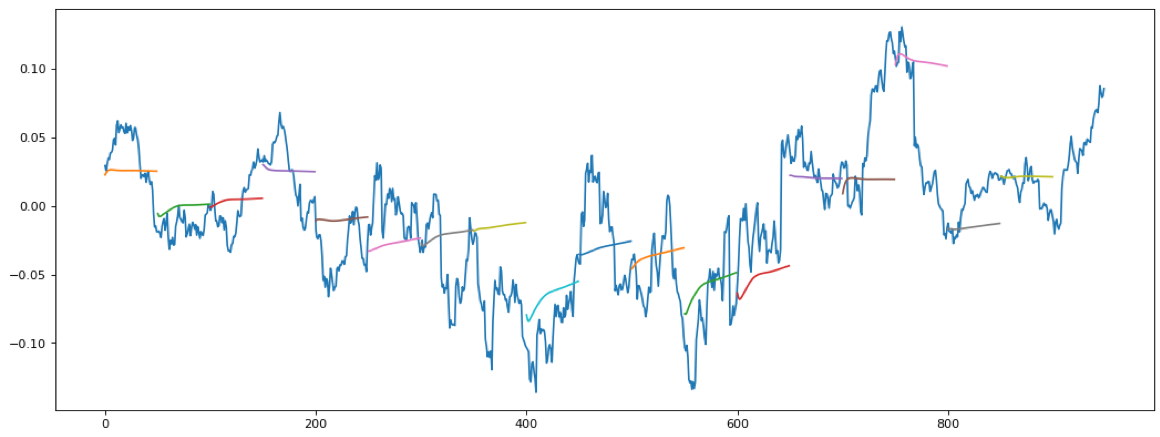
\includegraphics[width=0.9\textwidth]{./figs/SS_2_50.PNG}
\vspace{-0.2cm}
\caption{Sequence-by-Sequence prediction (2 Epoch, 50 Batch size)}
%\todo{fix scale from 1 to 41 and 1 to 100}}
\label{fig_predict}
\end{center}
\vspace{-0.6cm}
\end{figure}

\begin{figure}[htpb]
\begin{center}
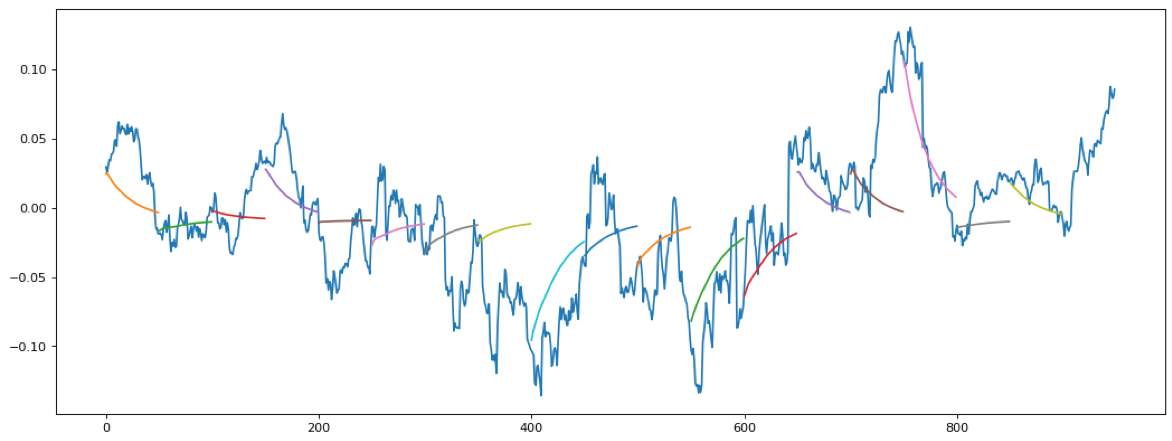
\includegraphics[width=0.9\textwidth]{./figs/SS_4_50.PNG}
\vspace{-0.2cm}
\caption{Sequence-by-Sequence prediction (4 Epoch, 50 Batch size)}
%\todo{fix scale from 1 to 41 and 1 to 100}}
\label{fig_predict}
\end{center}
\vspace{-0.6cm}
\end{figure}


\subsection{Effectiveness of using multiple features in NN model}

\begin{table}[htpb]
  %\scriptsize
  %\parbox{0.3\linewidth}{
  \centering
  \scalebox{0.85}{
  \begin{tabular}{||c| c | c | c ||}
  \hline\hline
  % Recall gives us an idea about when it’s actually yes, how often does it predict yes.
  % Precsion tells us about when it predicts yes, how often is it correct.
   Bar category & Precision & Recall & f1-score \\\hline
   1  & 0.82 & 0.73 & 0.77 \\\hline
   2  & 0.74 & 0.64 & 0.68\\\hline
   3  & 0.62 & 0.67 & 0.64\\\hline
   4  & 0.59 & 0.65 & 0.61\\\hline
   5  & 0.74 & 0.83 & 0.78\\\hline
   6  & 0.89 & 0.82 & 0.85\\\hline
   7  & 0.62 & 0.68 & 0.64\\\hline
   8  & 0.75 & 0.73 & 0.73\\\hline
   9  & 0.82 & 0.83 & 0.82\\\hline
   10 & 0.83 & 0.74 & 0.78\\\hline\hline

  \end{tabular}}
  \vspace{0.3cm}
  \caption{Accuracy of using multiple features in NN model}
  \label{table:features-acc}
  %}
\end{table}

In table \ref{table:features-acc} we describe the precision, recall and f1-score for using the different feature maps to predict different bar category. We divided all the bars into 10 different categories according to their shape. From table \ref{table:features-acc}, bar category 6 has the highest f1-score and category 3 and 7 has the lowest f1-score among all. Overall accuracy of our model is 67\%.
